\chapter[SCP-087 楼梯间]{
    SCP-087 The Stairwell\\
    SCP-087 楼梯间\\
    \heritage
}

\label{chap:SCP-087}

\begin{figure}[H]
    \centering
    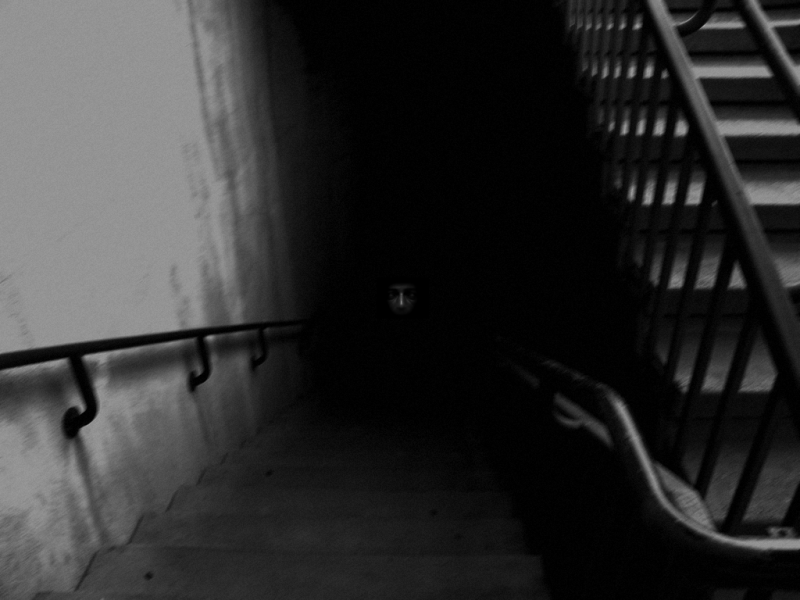
\includegraphics[width=0.5\linewidth]{images/SCP.087.png}
    \caption*{图片A,从第一次探索的录像中截取的静止帧。}
\end{figure}

\bb{项目编号:}SCP-087

\bb{项目等级:}Euclid

\bb{特殊收容措施:}SCP-087位于{[}已编辑]的校园内,通向SCP-087的门廊由带有带电封锁机制的强化钢板构筑而成,此入口已经被伪装成类似于与该建筑设计一致的门卫室。大门的封锁机制不会解除,除非同时施加██伏特的电流并逆时针扭转钥匙。在门的内部,有6厘米厚的工业泡沫填充。

因为最后一次探索的结果(参阅文件087-IV ),现在禁止任何人进入SCP-087。

\bb{描述:} SCP-087是一个无灯的平台楼梯,每层是斜38度的13阶楼梯,楼层之间是一个180度的大概直径3米的半圆平台,由于在SCP-087里面可见度只有1.5个阶梯,并且没有任何的壁灯和窗户,所以任何去探索SCP-087的人员必须配备照明设备,光源75瓦足够,超过75瓦不会有更好的照明效果,因为SCP-087似乎可以吸收过多的光线。

探索人员报告和声音记录证明项目中存在一种令人紧张的声音,类似于介于█岁至██岁孩童的哭声。估测此声音的来源大约位于首个楼梯平台下方200米处。然而,不管怎样继续前进,都不能感觉到在接近这个声音,从第4次探索(也是最后并且下行距离最远的一次)中看,深度是远远超出了现在科学的建筑和地址结构所能达到的深度。至今为止,仍然不能知道SCP-087到底有没有尽头。

\begin{figure}[H]
    \centering
    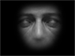
\includegraphics[width=0.5\linewidth]{images/SCP.087.2.png}
    \caption*{图片B,SCP-087-1,放大自第一次探索录像的静止画面。}
\end{figure}

SCP-087至今有4个由D级人员录制的探索录像,每个探险都遭遇到了SCP-087-1(SCP-087里面的未知物体),SCP-087-1是一张没有瞳孔,鼻和嘴的脸,SCP-087-1的性质是完全未知的,但是可以确定他不是哭泣声音的来源,当遇到SCP-087-1的时候,探索人员表现出强烈的疯狂和恐惧,但是很难知道这种反应是反常的还是简单的生理反应。

\bb{附录:}\\
当第4次探险结束后的两周, 有几位来自于{[}已编辑]大学的工作人员和学生都报告称听到SCP-087内部发出频率1-2秒\slash 次的敲击声。SCP-087门口被填充了6厘米的工业泡沫。之后不曾接到对敲击声的报告。

经授权的人员可以参阅文件087-I 到 087-IV,四次探索报告的文件。\\
\hyperref[chap:DOC-document-087-i]{文件087-I}\\
\hyperref[chap:DOC-document-087-ii]{文件087-II}\\
\hyperref[chap:DOC-document-087-iii]{文件087-III}\\
{[}资料被删除]
